
        \begin{figure}[H]
          
          \centering
          
  \begin{tikzpicture}
  \node at (1.5, 0.5){\color{blue}\faIcon{user}};
\fill[gray] (2, 0) rectangle (3, 1);
\fill[gray] (0, 1) rectangle (1, 2);
\fill[gray] (2, 1) rectangle (3, 2);
\fill[gray] (4, 1) rectangle (5, 2);
\fill[gray] (0, 2) rectangle (1, 3);
\fill[gray] (2, 2) rectangle (3, 3);
\fill[gray] (4, 2) rectangle (5, 3);
\node at (4.5, 3.5){\color{blue}\faIcon{home}};
\fill[gray] (0, 4) rectangle (1, 5);
\fill[gray] (1, 4) rectangle (2, 5);
\fill[gray] (3, 4) rectangle (4, 5);
\fill[gray] (4, 4) rectangle (5, 5);
\draw[black] grid (5, 5);
  \end{tikzpicture}
  
          \caption{Dodaj do kolejki węzeł x: 1 y: 0}
          \label{fig:astar_solve_steps}
        \end{figure}
        
        \begin{figure}[H]
          \ContinuedFloat
          \centering
          
  \begin{tikzpicture}
  \node at (1.5, 0.5){\color{blue}\faIcon{user}};
\fill[gray] (2, 0) rectangle (3, 1);
\fill[gray] (0, 1) rectangle (1, 2);
\fill[gray] (2, 1) rectangle (3, 2);
\fill[gray] (4, 1) rectangle (5, 2);
\fill[gray] (0, 2) rectangle (1, 3);
\fill[gray] (2, 2) rectangle (3, 3);
\fill[gray] (4, 2) rectangle (5, 3);
\node at (4.5, 3.5){\color{blue}\faIcon{home}};
\fill[gray] (0, 4) rectangle (1, 5);
\fill[gray] (1, 4) rectangle (2, 5);
\fill[gray] (3, 4) rectangle (4, 5);
\fill[gray] (4, 4) rectangle (5, 5);
\draw[black] grid (5, 5);
  \end{tikzpicture}
  
          \caption{Rozpatrz x: 1 y: 0}
          
        \end{figure}
        
        \begin{figure}[H]
          \ContinuedFloat
          \centering
          
  \begin{tikzpicture}
  \node at (1.5, 0.5){\color{blue}\faIcon{user}};
\fill[gray] (2, 0) rectangle (3, 1);
\fill[gray] (0, 1) rectangle (1, 2);
\node at (1.5, 1.5){\color{purple}\faIcon{hourglass}};
\fill[gray] (2, 1) rectangle (3, 2);
\fill[gray] (4, 1) rectangle (5, 2);
\fill[gray] (0, 2) rectangle (1, 3);
\fill[gray] (2, 2) rectangle (3, 3);
\fill[gray] (4, 2) rectangle (5, 3);
\node at (4.5, 3.5){\color{blue}\faIcon{home}};
\fill[gray] (0, 4) rectangle (1, 5);
\fill[gray] (1, 4) rectangle (2, 5);
\fill[gray] (3, 4) rectangle (4, 5);
\fill[gray] (4, 4) rectangle (5, 5);
\draw[black] grid (5, 5);
  \end{tikzpicture}
  
          \caption{Dodaj do kolejki węzeł x: 1 y: 1}
          
        \end{figure}
        
        \begin{figure}[H]
          \ContinuedFloat
          \centering
          
  \begin{tikzpicture}
  \node at (0.5, 0.5){\color{purple}\faIcon{hourglass}};
\node at (1.5, 0.5){\color{blue}\faIcon{user}};
\fill[gray] (2, 0) rectangle (3, 1);
\fill[gray] (0, 1) rectangle (1, 2);
\node at (1.5, 1.5){\color{purple}\faIcon{hourglass}};
\fill[gray] (2, 1) rectangle (3, 2);
\fill[gray] (4, 1) rectangle (5, 2);
\fill[gray] (0, 2) rectangle (1, 3);
\fill[gray] (2, 2) rectangle (3, 3);
\fill[gray] (4, 2) rectangle (5, 3);
\node at (4.5, 3.5){\color{blue}\faIcon{home}};
\fill[gray] (0, 4) rectangle (1, 5);
\fill[gray] (1, 4) rectangle (2, 5);
\fill[gray] (3, 4) rectangle (4, 5);
\fill[gray] (4, 4) rectangle (5, 5);
\draw[black] grid (5, 5);
  \end{tikzpicture}
  
          \caption{Dodaj do kolejki węzeł x: 0 y: 0}
          
        \end{figure}
        
        \begin{figure}[H]
          \ContinuedFloat
          \centering
          
  \begin{tikzpicture}
  \node at (0.5, 0.5){\color{purple}\faIcon{hourglass}};
\node at (1.5, 0.5){\color{blue}\faIcon{user}};
\fill[gray] (2, 0) rectangle (3, 1);
\fill[gray] (0, 1) rectangle (1, 2);
\node at (1.5, 1.5){\color{orange}\faIcon{arrows-alt}};
\fill[gray] (2, 1) rectangle (3, 2);
\fill[gray] (4, 1) rectangle (5, 2);
\fill[gray] (0, 2) rectangle (1, 3);
\fill[gray] (2, 2) rectangle (3, 3);
\fill[gray] (4, 2) rectangle (5, 3);
\node at (4.5, 3.5){\color{blue}\faIcon{home}};
\fill[gray] (0, 4) rectangle (1, 5);
\fill[gray] (1, 4) rectangle (2, 5);
\fill[gray] (3, 4) rectangle (4, 5);
\fill[gray] (4, 4) rectangle (5, 5);
\draw[black] grid (5, 5);
  \end{tikzpicture}
  
          \caption{Rozpatrz x: 1 y: 1}
          
        \end{figure}
        
        \begin{figure}[H]
          \ContinuedFloat
          \centering
          
  \begin{tikzpicture}
  \node at (0.5, 0.5){\color{purple}\faIcon{hourglass}};
\node at (1.5, 0.5){\color{blue}\faIcon{user}};
\fill[gray] (2, 0) rectangle (3, 1);
\fill[gray] (0, 1) rectangle (1, 2);
\node at (1.5, 1.5){\color{orange}\faIcon{arrows-alt}};
\fill[gray] (2, 1) rectangle (3, 2);
\fill[gray] (4, 1) rectangle (5, 2);
\fill[gray] (0, 2) rectangle (1, 3);
\node at (1.5, 2.5){\color{purple}\faIcon{hourglass}};
\fill[gray] (2, 2) rectangle (3, 3);
\fill[gray] (4, 2) rectangle (5, 3);
\node at (4.5, 3.5){\color{blue}\faIcon{home}};
\fill[gray] (0, 4) rectangle (1, 5);
\fill[gray] (1, 4) rectangle (2, 5);
\fill[gray] (3, 4) rectangle (4, 5);
\fill[gray] (4, 4) rectangle (5, 5);
\draw[black] grid (5, 5);
  \end{tikzpicture}
  
          \caption{Dodaj do kolejki węzeł x: 1 y: 2}
          
        \end{figure}
        
        \begin{figure}[H]
          \ContinuedFloat
          \centering
          
  \begin{tikzpicture}
  \node at (0.5, 0.5){\color{purple}\faIcon{hourglass}};
\node at (1.5, 0.5){\color{blue}\faIcon{user}};
\fill[gray] (2, 0) rectangle (3, 1);
\fill[gray] (0, 1) rectangle (1, 2);
\node at (1.5, 1.5){\color{orange}\faIcon{arrows-alt}};
\fill[gray] (2, 1) rectangle (3, 2);
\fill[gray] (4, 1) rectangle (5, 2);
\fill[gray] (0, 2) rectangle (1, 3);
\node at (1.5, 2.5){\color{orange}\faIcon{arrows-alt}};
\fill[gray] (2, 2) rectangle (3, 3);
\fill[gray] (4, 2) rectangle (5, 3);
\node at (4.5, 3.5){\color{blue}\faIcon{home}};
\fill[gray] (0, 4) rectangle (1, 5);
\fill[gray] (1, 4) rectangle (2, 5);
\fill[gray] (3, 4) rectangle (4, 5);
\fill[gray] (4, 4) rectangle (5, 5);
\draw[black] grid (5, 5);
  \end{tikzpicture}
  
          \caption{Rozpatrz x: 1 y: 2}
          
        \end{figure}
        
        \begin{figure}[H]
          \ContinuedFloat
          \centering
          
  \begin{tikzpicture}
  \node at (0.5, 0.5){\color{purple}\faIcon{hourglass}};
\node at (1.5, 0.5){\color{blue}\faIcon{user}};
\fill[gray] (2, 0) rectangle (3, 1);
\fill[gray] (0, 1) rectangle (1, 2);
\node at (1.5, 1.5){\color{orange}\faIcon{arrows-alt}};
\fill[gray] (2, 1) rectangle (3, 2);
\fill[gray] (4, 1) rectangle (5, 2);
\fill[gray] (0, 2) rectangle (1, 3);
\node at (1.5, 2.5){\color{orange}\faIcon{arrows-alt}};
\fill[gray] (2, 2) rectangle (3, 3);
\fill[gray] (4, 2) rectangle (5, 3);
\node at (1.5, 3.5){\color{purple}\faIcon{hourglass}};
\node at (4.5, 3.5){\color{blue}\faIcon{home}};
\fill[gray] (0, 4) rectangle (1, 5);
\fill[gray] (1, 4) rectangle (2, 5);
\fill[gray] (3, 4) rectangle (4, 5);
\fill[gray] (4, 4) rectangle (5, 5);
\draw[black] grid (5, 5);
  \end{tikzpicture}
  
          \caption{Dodaj do kolejki węzeł x: 1 y: 3}
          
        \end{figure}
        
        \begin{figure}[H]
          \ContinuedFloat
          \centering
          
  \begin{tikzpicture}
  \node at (0.5, 0.5){\color{purple}\faIcon{hourglass}};
\node at (1.5, 0.5){\color{blue}\faIcon{user}};
\fill[gray] (2, 0) rectangle (3, 1);
\fill[gray] (0, 1) rectangle (1, 2);
\node at (1.5, 1.5){\color{orange}\faIcon{arrows-alt}};
\fill[gray] (2, 1) rectangle (3, 2);
\fill[gray] (4, 1) rectangle (5, 2);
\fill[gray] (0, 2) rectangle (1, 3);
\node at (1.5, 2.5){\color{orange}\faIcon{arrows-alt}};
\fill[gray] (2, 2) rectangle (3, 3);
\fill[gray] (4, 2) rectangle (5, 3);
\node at (1.5, 3.5){\color{orange}\faIcon{arrows-alt}};
\node at (4.5, 3.5){\color{blue}\faIcon{home}};
\fill[gray] (0, 4) rectangle (1, 5);
\fill[gray] (1, 4) rectangle (2, 5);
\fill[gray] (3, 4) rectangle (4, 5);
\fill[gray] (4, 4) rectangle (5, 5);
\draw[black] grid (5, 5);
  \end{tikzpicture}
  
          \caption{Rozpatrz x: 1 y: 3}
          
        \end{figure}
        
        \begin{figure}[H]
          \ContinuedFloat
          \centering
          
  \begin{tikzpicture}
  \node at (0.5, 0.5){\color{purple}\faIcon{hourglass}};
\node at (1.5, 0.5){\color{blue}\faIcon{user}};
\fill[gray] (2, 0) rectangle (3, 1);
\fill[gray] (0, 1) rectangle (1, 2);
\node at (1.5, 1.5){\color{orange}\faIcon{arrows-alt}};
\fill[gray] (2, 1) rectangle (3, 2);
\fill[gray] (4, 1) rectangle (5, 2);
\fill[gray] (0, 2) rectangle (1, 3);
\node at (1.5, 2.5){\color{orange}\faIcon{arrows-alt}};
\fill[gray] (2, 2) rectangle (3, 3);
\fill[gray] (4, 2) rectangle (5, 3);
\node at (0.5, 3.5){\color{purple}\faIcon{hourglass}};
\node at (1.5, 3.5){\color{orange}\faIcon{arrows-alt}};
\node at (4.5, 3.5){\color{blue}\faIcon{home}};
\fill[gray] (0, 4) rectangle (1, 5);
\fill[gray] (1, 4) rectangle (2, 5);
\fill[gray] (3, 4) rectangle (4, 5);
\fill[gray] (4, 4) rectangle (5, 5);
\draw[black] grid (5, 5);
  \end{tikzpicture}
  
          \caption{Dodaj do kolejki węzeł x: 0 y: 3}
          
        \end{figure}
        
        \begin{figure}[H]
          \ContinuedFloat
          \centering
          
  \begin{tikzpicture}
  \node at (0.5, 0.5){\color{purple}\faIcon{hourglass}};
\node at (1.5, 0.5){\color{blue}\faIcon{user}};
\fill[gray] (2, 0) rectangle (3, 1);
\fill[gray] (0, 1) rectangle (1, 2);
\node at (1.5, 1.5){\color{orange}\faIcon{arrows-alt}};
\fill[gray] (2, 1) rectangle (3, 2);
\fill[gray] (4, 1) rectangle (5, 2);
\fill[gray] (0, 2) rectangle (1, 3);
\node at (1.5, 2.5){\color{orange}\faIcon{arrows-alt}};
\fill[gray] (2, 2) rectangle (3, 3);
\fill[gray] (4, 2) rectangle (5, 3);
\node at (0.5, 3.5){\color{purple}\faIcon{hourglass}};
\node at (1.5, 3.5){\color{orange}\faIcon{arrows-alt}};
\node at (2.5, 3.5){\color{purple}\faIcon{hourglass}};
\node at (4.5, 3.5){\color{blue}\faIcon{home}};
\fill[gray] (0, 4) rectangle (1, 5);
\fill[gray] (1, 4) rectangle (2, 5);
\fill[gray] (3, 4) rectangle (4, 5);
\fill[gray] (4, 4) rectangle (5, 5);
\draw[black] grid (5, 5);
  \end{tikzpicture}
  
          \caption{Dodaj do kolejki węzeł x: 2 y: 3}
          
        \end{figure}
        
        \begin{figure}[H]
          \ContinuedFloat
          \centering
          
  \begin{tikzpicture}
  \node at (0.5, 0.5){\color{purple}\faIcon{hourglass}};
\node at (1.5, 0.5){\color{blue}\faIcon{user}};
\fill[gray] (2, 0) rectangle (3, 1);
\fill[gray] (0, 1) rectangle (1, 2);
\node at (1.5, 1.5){\color{orange}\faIcon{arrows-alt}};
\fill[gray] (2, 1) rectangle (3, 2);
\fill[gray] (4, 1) rectangle (5, 2);
\fill[gray] (0, 2) rectangle (1, 3);
\node at (1.5, 2.5){\color{orange}\faIcon{arrows-alt}};
\fill[gray] (2, 2) rectangle (3, 3);
\fill[gray] (4, 2) rectangle (5, 3);
\node at (0.5, 3.5){\color{purple}\faIcon{hourglass}};
\node at (1.5, 3.5){\color{orange}\faIcon{arrows-alt}};
\node at (2.5, 3.5){\color{orange}\faIcon{arrows-alt}};
\node at (4.5, 3.5){\color{blue}\faIcon{home}};
\fill[gray] (0, 4) rectangle (1, 5);
\fill[gray] (1, 4) rectangle (2, 5);
\fill[gray] (3, 4) rectangle (4, 5);
\fill[gray] (4, 4) rectangle (5, 5);
\draw[black] grid (5, 5);
  \end{tikzpicture}
  
          \caption{Rozpatrz x: 2 y: 3}
          
        \end{figure}
        
        \begin{figure}[H]
          \ContinuedFloat
          \centering
          
  \begin{tikzpicture}
  \node at (0.5, 0.5){\color{purple}\faIcon{hourglass}};
\node at (1.5, 0.5){\color{blue}\faIcon{user}};
\fill[gray] (2, 0) rectangle (3, 1);
\fill[gray] (0, 1) rectangle (1, 2);
\node at (1.5, 1.5){\color{orange}\faIcon{arrows-alt}};
\fill[gray] (2, 1) rectangle (3, 2);
\fill[gray] (4, 1) rectangle (5, 2);
\fill[gray] (0, 2) rectangle (1, 3);
\node at (1.5, 2.5){\color{orange}\faIcon{arrows-alt}};
\fill[gray] (2, 2) rectangle (3, 3);
\fill[gray] (4, 2) rectangle (5, 3);
\node at (0.5, 3.5){\color{purple}\faIcon{hourglass}};
\node at (1.5, 3.5){\color{orange}\faIcon{arrows-alt}};
\node at (2.5, 3.5){\color{orange}\faIcon{arrows-alt}};
\node at (4.5, 3.5){\color{blue}\faIcon{home}};
\fill[gray] (0, 4) rectangle (1, 5);
\fill[gray] (1, 4) rectangle (2, 5);
\node at (2.5, 4.5){\color{purple}\faIcon{hourglass}};
\fill[gray] (3, 4) rectangle (4, 5);
\fill[gray] (4, 4) rectangle (5, 5);
\draw[black] grid (5, 5);
  \end{tikzpicture}
  
          \caption{Dodaj do kolejki węzeł x: 2 y: 4}
          
        \end{figure}
        
        \begin{figure}[H]
          \ContinuedFloat
          \centering
          
  \begin{tikzpicture}
  \node at (0.5, 0.5){\color{purple}\faIcon{hourglass}};
\node at (1.5, 0.5){\color{blue}\faIcon{user}};
\fill[gray] (2, 0) rectangle (3, 1);
\fill[gray] (0, 1) rectangle (1, 2);
\node at (1.5, 1.5){\color{orange}\faIcon{arrows-alt}};
\fill[gray] (2, 1) rectangle (3, 2);
\fill[gray] (4, 1) rectangle (5, 2);
\fill[gray] (0, 2) rectangle (1, 3);
\node at (1.5, 2.5){\color{orange}\faIcon{arrows-alt}};
\fill[gray] (2, 2) rectangle (3, 3);
\fill[gray] (4, 2) rectangle (5, 3);
\node at (0.5, 3.5){\color{purple}\faIcon{hourglass}};
\node at (1.5, 3.5){\color{orange}\faIcon{arrows-alt}};
\node at (2.5, 3.5){\color{orange}\faIcon{arrows-alt}};
\node at (3.5, 3.5){\color{purple}\faIcon{hourglass}};
\node at (4.5, 3.5){\color{blue}\faIcon{home}};
\fill[gray] (0, 4) rectangle (1, 5);
\fill[gray] (1, 4) rectangle (2, 5);
\node at (2.5, 4.5){\color{purple}\faIcon{hourglass}};
\fill[gray] (3, 4) rectangle (4, 5);
\fill[gray] (4, 4) rectangle (5, 5);
\draw[black] grid (5, 5);
  \end{tikzpicture}
  
          \caption{Dodaj do kolejki węzeł x: 3 y: 3}
          
        \end{figure}
        
        \begin{figure}[H]
          \ContinuedFloat
          \centering
          
  \begin{tikzpicture}
  \node at (0.5, 0.5){\color{purple}\faIcon{hourglass}};
\node at (1.5, 0.5){\color{blue}\faIcon{user}};
\fill[gray] (2, 0) rectangle (3, 1);
\fill[gray] (0, 1) rectangle (1, 2);
\node at (1.5, 1.5){\color{orange}\faIcon{arrows-alt}};
\fill[gray] (2, 1) rectangle (3, 2);
\fill[gray] (4, 1) rectangle (5, 2);
\fill[gray] (0, 2) rectangle (1, 3);
\node at (1.5, 2.5){\color{orange}\faIcon{arrows-alt}};
\fill[gray] (2, 2) rectangle (3, 3);
\fill[gray] (4, 2) rectangle (5, 3);
\node at (0.5, 3.5){\color{purple}\faIcon{hourglass}};
\node at (1.5, 3.5){\color{orange}\faIcon{arrows-alt}};
\node at (2.5, 3.5){\color{orange}\faIcon{arrows-alt}};
\node at (3.5, 3.5){\color{orange}\faIcon{arrows-alt}};
\node at (4.5, 3.5){\color{blue}\faIcon{home}};
\fill[gray] (0, 4) rectangle (1, 5);
\fill[gray] (1, 4) rectangle (2, 5);
\node at (2.5, 4.5){\color{purple}\faIcon{hourglass}};
\fill[gray] (3, 4) rectangle (4, 5);
\fill[gray] (4, 4) rectangle (5, 5);
\draw[black] grid (5, 5);
  \end{tikzpicture}
  
          \caption{Rozpatrz x: 3 y: 3}
          
        \end{figure}
        
        \begin{figure}[H]
          \ContinuedFloat
          \centering
          
  \begin{tikzpicture}
  \node at (0.5, 0.5){\color{purple}\faIcon{hourglass}};
\node at (1.5, 0.5){\color{blue}\faIcon{user}};
\fill[gray] (2, 0) rectangle (3, 1);
\fill[gray] (0, 1) rectangle (1, 2);
\node at (1.5, 1.5){\color{orange}\faIcon{arrows-alt}};
\fill[gray] (2, 1) rectangle (3, 2);
\fill[gray] (4, 1) rectangle (5, 2);
\fill[gray] (0, 2) rectangle (1, 3);
\node at (1.5, 2.5){\color{orange}\faIcon{arrows-alt}};
\fill[gray] (2, 2) rectangle (3, 3);
\node at (3.5, 2.5){\color{purple}\faIcon{hourglass}};
\fill[gray] (4, 2) rectangle (5, 3);
\node at (0.5, 3.5){\color{purple}\faIcon{hourglass}};
\node at (1.5, 3.5){\color{orange}\faIcon{arrows-alt}};
\node at (2.5, 3.5){\color{orange}\faIcon{arrows-alt}};
\node at (3.5, 3.5){\color{orange}\faIcon{arrows-alt}};
\node at (4.5, 3.5){\color{blue}\faIcon{home}};
\fill[gray] (0, 4) rectangle (1, 5);
\fill[gray] (1, 4) rectangle (2, 5);
\node at (2.5, 4.5){\color{purple}\faIcon{hourglass}};
\fill[gray] (3, 4) rectangle (4, 5);
\fill[gray] (4, 4) rectangle (5, 5);
\draw[black] grid (5, 5);
  \end{tikzpicture}
  
          \caption{Dodaj do kolejki węzeł x: 3 y: 2}
          
        \end{figure}
        
        \begin{figure}[H]
          \ContinuedFloat
          \centering
          
  \begin{tikzpicture}
  \node at (0.5, 0.5){\color{purple}\faIcon{hourglass}};
\node at (1.5, 0.5){\color{blue}\faIcon{user}};
\fill[gray] (2, 0) rectangle (3, 1);
\fill[gray] (0, 1) rectangle (1, 2);
\node at (1.5, 1.5){\color{orange}\faIcon{arrows-alt}};
\fill[gray] (2, 1) rectangle (3, 2);
\fill[gray] (4, 1) rectangle (5, 2);
\fill[gray] (0, 2) rectangle (1, 3);
\node at (1.5, 2.5){\color{orange}\faIcon{arrows-alt}};
\fill[gray] (2, 2) rectangle (3, 3);
\node at (3.5, 2.5){\color{purple}\faIcon{hourglass}};
\fill[gray] (4, 2) rectangle (5, 3);
\node at (0.5, 3.5){\color{purple}\faIcon{hourglass}};
\node at (1.5, 3.5){\color{orange}\faIcon{arrows-alt}};
\node at (2.5, 3.5){\color{orange}\faIcon{arrows-alt}};
\node at (3.5, 3.5){\color{orange}\faIcon{arrows-alt}};
\node at (4.5, 3.5){\color{blue}\faIcon{home}};
\fill[gray] (0, 4) rectangle (1, 5);
\fill[gray] (1, 4) rectangle (2, 5);
\node at (2.5, 4.5){\color{purple}\faIcon{hourglass}};
\fill[gray] (3, 4) rectangle (4, 5);
\fill[gray] (4, 4) rectangle (5, 5);
\draw[black] grid (5, 5);
  \end{tikzpicture}
  
          \caption{Dodaj do kolejki węzeł x: 4 y: 3}
          
        \end{figure}
        
        \begin{figure}[H]
          \ContinuedFloat
          \centering
          
  \begin{tikzpicture}
  \node at (0.5, 0.5){\color{purple}\faIcon{hourglass}};
\node at (1.5, 0.5){\color{blue}\faIcon{user}};
\fill[gray] (2, 0) rectangle (3, 1);
\fill[gray] (0, 1) rectangle (1, 2);
\node at (1.5, 1.5){\color{orange}\faIcon{arrows-alt}};
\fill[gray] (2, 1) rectangle (3, 2);
\fill[gray] (4, 1) rectangle (5, 2);
\fill[gray] (0, 2) rectangle (1, 3);
\node at (1.5, 2.5){\color{orange}\faIcon{arrows-alt}};
\fill[gray] (2, 2) rectangle (3, 3);
\node at (3.5, 2.5){\color{purple}\faIcon{hourglass}};
\fill[gray] (4, 2) rectangle (5, 3);
\node at (0.5, 3.5){\color{purple}\faIcon{hourglass}};
\node at (1.5, 3.5){\color{orange}\faIcon{arrows-alt}};
\node at (2.5, 3.5){\color{orange}\faIcon{arrows-alt}};
\node at (3.5, 3.5){\color{orange}\faIcon{arrows-alt}};
\node at (4.5, 3.5){\color{blue}\faIcon{home}};
\fill[gray] (0, 4) rectangle (1, 5);
\fill[gray] (1, 4) rectangle (2, 5);
\node at (2.5, 4.5){\color{purple}\faIcon{hourglass}};
\fill[gray] (3, 4) rectangle (4, 5);
\fill[gray] (4, 4) rectangle (5, 5);
\draw[black] grid (5, 5);
  \end{tikzpicture}
  
          \caption{Rozpatrz x: 4 y: 3}
          
        \end{figure}
        
        \begin{figure}[H]
          \ContinuedFloat
          \centering
          
  \begin{tikzpicture}
  \node at (0.5, 0.5){\color{purple}\faIcon{hourglass}};
\node at (1.5, 0.5){\color{blue}\faIcon{user}};
\fill[gray] (2, 0) rectangle (3, 1);
\fill[gray] (0, 1) rectangle (1, 2);
\node at (1.5, 1.5){\color{orange}\faIcon{arrows-alt}};
\fill[gray] (2, 1) rectangle (3, 2);
\fill[gray] (4, 1) rectangle (5, 2);
\fill[gray] (0, 2) rectangle (1, 3);
\node at (1.5, 2.5){\color{orange}\faIcon{arrows-alt}};
\fill[gray] (2, 2) rectangle (3, 3);
\node at (3.5, 2.5){\color{purple}\faIcon{hourglass}};
\fill[gray] (4, 2) rectangle (5, 3);
\node at (0.5, 3.5){\color{purple}\faIcon{hourglass}};
\node at (1.5, 3.5){\color{orange}\faIcon{arrows-alt}};
\node at (2.5, 3.5){\color{orange}\faIcon{arrows-alt}};
\node at (3.5, 3.5){\color{orange}\faIcon{arrows-alt}};
\node at (4.5, 3.5){\color{blue}\faIcon{home}};
\fill[gray] (0, 4) rectangle (1, 5);
\fill[gray] (1, 4) rectangle (2, 5);
\node at (2.5, 4.5){\color{purple}\faIcon{hourglass}};
\fill[gray] (3, 4) rectangle (4, 5);
\fill[gray] (4, 4) rectangle (5, 5);
\draw[black] grid (5, 5);
  \end{tikzpicture}
  
          \caption{Wybierz x: 4 y: 3 do finalnej ścierzki}
          
        \end{figure}
        
        \begin{figure}[H]
          \ContinuedFloat
          \centering
          
  \begin{tikzpicture}
  \node at (0.5, 0.5){\color{purple}\faIcon{hourglass}};
\node at (1.5, 0.5){\color{blue}\faIcon{user}};
\fill[gray] (2, 0) rectangle (3, 1);
\fill[gray] (0, 1) rectangle (1, 2);
\node at (1.5, 1.5){\color{orange}\faIcon{arrows-alt}};
\fill[gray] (2, 1) rectangle (3, 2);
\fill[gray] (4, 1) rectangle (5, 2);
\fill[gray] (0, 2) rectangle (1, 3);
\node at (1.5, 2.5){\color{orange}\faIcon{arrows-alt}};
\fill[gray] (2, 2) rectangle (3, 3);
\node at (3.5, 2.5){\color{purple}\faIcon{hourglass}};
\fill[gray] (4, 2) rectangle (5, 3);
\node at (0.5, 3.5){\color{purple}\faIcon{hourglass}};
\node at (1.5, 3.5){\color{orange}\faIcon{arrows-alt}};
\node at (2.5, 3.5){\color{orange}\faIcon{arrows-alt}};
\node at (3.5, 3.5){\color{green}\faIcon{check}};
\node at (4.5, 3.5){\color{blue}\faIcon{home}};
\fill[gray] (0, 4) rectangle (1, 5);
\fill[gray] (1, 4) rectangle (2, 5);
\node at (2.5, 4.5){\color{purple}\faIcon{hourglass}};
\fill[gray] (3, 4) rectangle (4, 5);
\fill[gray] (4, 4) rectangle (5, 5);
\draw[black] grid (5, 5);
  \end{tikzpicture}
  
          \caption{Wybierz x: 3 y: 3 do finalnej ścierzki}
          
        \end{figure}
        
        \begin{figure}[H]
          \ContinuedFloat
          \centering
          
  \begin{tikzpicture}
  \node at (0.5, 0.5){\color{purple}\faIcon{hourglass}};
\node at (1.5, 0.5){\color{blue}\faIcon{user}};
\fill[gray] (2, 0) rectangle (3, 1);
\fill[gray] (0, 1) rectangle (1, 2);
\node at (1.5, 1.5){\color{orange}\faIcon{arrows-alt}};
\fill[gray] (2, 1) rectangle (3, 2);
\fill[gray] (4, 1) rectangle (5, 2);
\fill[gray] (0, 2) rectangle (1, 3);
\node at (1.5, 2.5){\color{orange}\faIcon{arrows-alt}};
\fill[gray] (2, 2) rectangle (3, 3);
\node at (3.5, 2.5){\color{purple}\faIcon{hourglass}};
\fill[gray] (4, 2) rectangle (5, 3);
\node at (0.5, 3.5){\color{purple}\faIcon{hourglass}};
\node at (1.5, 3.5){\color{orange}\faIcon{arrows-alt}};
\node at (2.5, 3.5){\color{green}\faIcon{check}};
\node at (3.5, 3.5){\color{green}\faIcon{check}};
\node at (4.5, 3.5){\color{blue}\faIcon{home}};
\fill[gray] (0, 4) rectangle (1, 5);
\fill[gray] (1, 4) rectangle (2, 5);
\node at (2.5, 4.5){\color{purple}\faIcon{hourglass}};
\fill[gray] (3, 4) rectangle (4, 5);
\fill[gray] (4, 4) rectangle (5, 5);
\draw[black] grid (5, 5);
  \end{tikzpicture}
  
          \caption{Wybierz x: 2 y: 3 do finalnej ścierzki}
          
        \end{figure}
        
        \begin{figure}[H]
          \ContinuedFloat
          \centering
          
  \begin{tikzpicture}
  \node at (0.5, 0.5){\color{purple}\faIcon{hourglass}};
\node at (1.5, 0.5){\color{blue}\faIcon{user}};
\fill[gray] (2, 0) rectangle (3, 1);
\fill[gray] (0, 1) rectangle (1, 2);
\node at (1.5, 1.5){\color{orange}\faIcon{arrows-alt}};
\fill[gray] (2, 1) rectangle (3, 2);
\fill[gray] (4, 1) rectangle (5, 2);
\fill[gray] (0, 2) rectangle (1, 3);
\node at (1.5, 2.5){\color{orange}\faIcon{arrows-alt}};
\fill[gray] (2, 2) rectangle (3, 3);
\node at (3.5, 2.5){\color{purple}\faIcon{hourglass}};
\fill[gray] (4, 2) rectangle (5, 3);
\node at (0.5, 3.5){\color{purple}\faIcon{hourglass}};
\node at (1.5, 3.5){\color{green}\faIcon{check}};
\node at (2.5, 3.5){\color{green}\faIcon{check}};
\node at (3.5, 3.5){\color{green}\faIcon{check}};
\node at (4.5, 3.5){\color{blue}\faIcon{home}};
\fill[gray] (0, 4) rectangle (1, 5);
\fill[gray] (1, 4) rectangle (2, 5);
\node at (2.5, 4.5){\color{purple}\faIcon{hourglass}};
\fill[gray] (3, 4) rectangle (4, 5);
\fill[gray] (4, 4) rectangle (5, 5);
\draw[black] grid (5, 5);
  \end{tikzpicture}
  
          \caption{Wybierz x: 1 y: 3 do finalnej ścierzki}
          
        \end{figure}
        
        \begin{figure}[H]
          \ContinuedFloat
          \centering
          
  \begin{tikzpicture}
  \node at (0.5, 0.5){\color{purple}\faIcon{hourglass}};
\node at (1.5, 0.5){\color{blue}\faIcon{user}};
\fill[gray] (2, 0) rectangle (3, 1);
\fill[gray] (0, 1) rectangle (1, 2);
\node at (1.5, 1.5){\color{orange}\faIcon{arrows-alt}};
\fill[gray] (2, 1) rectangle (3, 2);
\fill[gray] (4, 1) rectangle (5, 2);
\fill[gray] (0, 2) rectangle (1, 3);
\node at (1.5, 2.5){\color{green}\faIcon{check}};
\fill[gray] (2, 2) rectangle (3, 3);
\node at (3.5, 2.5){\color{purple}\faIcon{hourglass}};
\fill[gray] (4, 2) rectangle (5, 3);
\node at (0.5, 3.5){\color{purple}\faIcon{hourglass}};
\node at (1.5, 3.5){\color{green}\faIcon{check}};
\node at (2.5, 3.5){\color{green}\faIcon{check}};
\node at (3.5, 3.5){\color{green}\faIcon{check}};
\node at (4.5, 3.5){\color{blue}\faIcon{home}};
\fill[gray] (0, 4) rectangle (1, 5);
\fill[gray] (1, 4) rectangle (2, 5);
\node at (2.5, 4.5){\color{purple}\faIcon{hourglass}};
\fill[gray] (3, 4) rectangle (4, 5);
\fill[gray] (4, 4) rectangle (5, 5);
\draw[black] grid (5, 5);
  \end{tikzpicture}
  
          \caption{Wybierz x: 1 y: 2 do finalnej ścierzki}
          
        \end{figure}
        
        \begin{figure}[H]
          \ContinuedFloat
          \centering
          
  \begin{tikzpicture}
  \node at (0.5, 0.5){\color{purple}\faIcon{hourglass}};
\node at (1.5, 0.5){\color{blue}\faIcon{user}};
\fill[gray] (2, 0) rectangle (3, 1);
\fill[gray] (0, 1) rectangle (1, 2);
\node at (1.5, 1.5){\color{green}\faIcon{check}};
\fill[gray] (2, 1) rectangle (3, 2);
\fill[gray] (4, 1) rectangle (5, 2);
\fill[gray] (0, 2) rectangle (1, 3);
\node at (1.5, 2.5){\color{green}\faIcon{check}};
\fill[gray] (2, 2) rectangle (3, 3);
\node at (3.5, 2.5){\color{purple}\faIcon{hourglass}};
\fill[gray] (4, 2) rectangle (5, 3);
\node at (0.5, 3.5){\color{purple}\faIcon{hourglass}};
\node at (1.5, 3.5){\color{green}\faIcon{check}};
\node at (2.5, 3.5){\color{green}\faIcon{check}};
\node at (3.5, 3.5){\color{green}\faIcon{check}};
\node at (4.5, 3.5){\color{blue}\faIcon{home}};
\fill[gray] (0, 4) rectangle (1, 5);
\fill[gray] (1, 4) rectangle (2, 5);
\node at (2.5, 4.5){\color{purple}\faIcon{hourglass}};
\fill[gray] (3, 4) rectangle (4, 5);
\fill[gray] (4, 4) rectangle (5, 5);
\draw[black] grid (5, 5);
  \end{tikzpicture}
  
          \caption{Wybierz x: 1 y: 1 do finalnej ścierzki}
          
        \end{figure}
        
        \begin{figure}[H]
          \ContinuedFloat
          \centering
          
  \begin{tikzpicture}
  \node at (0.5, 0.5){\color{purple}\faIcon{hourglass}};
\node at (1.5, 0.5){\color{blue}\faIcon{user}};
\fill[gray] (2, 0) rectangle (3, 1);
\fill[gray] (0, 1) rectangle (1, 2);
\node at (1.5, 1.5){\color{green}\faIcon{check}};
\fill[gray] (2, 1) rectangle (3, 2);
\fill[gray] (4, 1) rectangle (5, 2);
\fill[gray] (0, 2) rectangle (1, 3);
\node at (1.5, 2.5){\color{green}\faIcon{check}};
\fill[gray] (2, 2) rectangle (3, 3);
\node at (3.5, 2.5){\color{purple}\faIcon{hourglass}};
\fill[gray] (4, 2) rectangle (5, 3);
\node at (0.5, 3.5){\color{purple}\faIcon{hourglass}};
\node at (1.5, 3.5){\color{green}\faIcon{check}};
\node at (2.5, 3.5){\color{green}\faIcon{check}};
\node at (3.5, 3.5){\color{green}\faIcon{check}};
\node at (4.5, 3.5){\color{blue}\faIcon{home}};
\fill[gray] (0, 4) rectangle (1, 5);
\fill[gray] (1, 4) rectangle (2, 5);
\node at (2.5, 4.5){\color{purple}\faIcon{hourglass}};
\fill[gray] (3, 4) rectangle (4, 5);
\fill[gray] (4, 4) rectangle (5, 5);
\draw[black] grid (5, 5);
  \end{tikzpicture}
  
          \caption{Wybierz x: 1 y: 0 do finalnej ścierzki}
          
        \end{figure}
        